\documentclass[abstract=on,10pt,a4paper,bibliography=totocnumbered]{article}
\usepackage[paper=a4paper,left=35mm,right=35mm,top=25mm,bottom=30mm]{geometry}
\usepackage[doublespacing]{setspace}
\usepackage[english]{babel}
\usepackage[utf8]{inputenc}
\usepackage[round]{natbib}
% \usepackage[autostyle]{csquotes}
% \usepackage[
%     backend=biber,
%     style=authoryear-icomp,
%     natbib=true,
%     maxcitenames=1,
%     maxbibnames=99,
%     uniquelist=false,
%     url=true,
%     % doi=true,
%     doi=false,
%     isbn=true,
%     eprint=false,
%     sorting=nyt,
%     sortcites=false
% ]{biblatex}
% \addbibresource{Literature.bib}
\usepackage{amsmath}
\usepackage{colortbl}
\usepackage{amsfonts}
\usepackage{amssymb}
\usepackage{textcomp, gensymb}
\usepackage{gensymb}
\usepackage{graphicx}
\usepackage{tikz}
\usepackage{enumerate}
\usepackage{enumitem}
\usepackage{subcaption}
\usepackage{booktabs}
\usepackage[colorlinks, allcolors=black, urlcolor=blue]{hyperref}
\usepackage[nameinlink]{cleveref}
% \usepackage{lineno}
\usepackage{multirow}
\usepackage{arydshln}
\usepackage[flushleft]{threeparttable}
% \usepackage[nomarkers, nolists]{endfloat}
\usepackage[colorinlistoftodos]{todonotes}
\usepackage{scalerel}
\usepackage{tikz}
\usepackage{makecell}
\usetikzlibrary{svg.path}

%------------------------------------------------------------------------------
%	Some Styling
%------------------------------------------------------------------------------
% Creating some TikZ styles
\tikzset{
  nonterminal/.style = {rectangle
    , minimum size = 6mm
    , very thick
    , draw = black!
  }
}

% Changing the style of captions in figures etc.
\captionsetup{labelfont=bf, format=plain, font=small}

% Change how equations are referenced
\renewcommand{\theequation}{Equation \arabic{equation}}%

% % Remove some stuff we dont want to list
% \AtEveryBibitem{%
%   \clearfield{month}
%   \clearfield{day}
%   \clearfield{number}
%   \ifentrytype{article}{
%       \clearfield{url}
%       \clearfield{issn}
%       \clearfield{urlyear}
%   }{}
% }
%
% To be able to put an ORCID
\definecolor{orcidlogocol}{HTML}{A6CE39}
\tikzset{
  orcidlogo/.pic={
    \fill[orcidlogocol] svg{M256,128c0,70.7-57.3,128-128,128C57.3,256,0,198.7,0,128C0,57.3,57.3,0,128,0C198.7,0,256,57.3,256,128z};
    \fill[white] svg{M86.3,186.2H70.9V79.1h15.4v48.4V186.2z}
                 svg{M108.9,79.1h41.6c39.6,0,57,28.3,57,53.6c0,27.5-21.5,53.6-56.8,53.6h-41.8V79.1z M124.3,172.4h24.5c34.9,0,42.9-26.5,42.9-39.7c0-21.5-13.7-39.7-43.7-39.7h-23.7V172.4z}
                 svg{M88.7,56.8c0,5.5-4.5,10.1-10.1,10.1c-5.6,0-10.1-4.6-10.1-10.1c0-5.6,4.5-10.1,10.1-10.1C84.2,46.7,88.7,51.3,88.7,56.8z};
  }
}
\newcommand\orcid[1]{\href{https://orcid.org/#1}{\mbox{\scalerel*{

\begin{tikzpicture}[yscale=-1,transform shape]
  \pic{orcidlogo};
\end{tikzpicture}
}{|}}}}

\newcommand{\inputy}[1]{\input{#1}\unskip}

%------------------------------------------------------------------------------
%	Titlepage: Header
%------------------------------------------------------------------------------
\title{Simulating Dispersal across Seasonal Landscapes to Assess Dynamic
Connectivity for an Endangered Large Carnivore}

% List of Authors
\author{
  David D. Hofmann\textsuperscript{1,2,\S} \orcid{0000-0003-3477-4365} \and
  Dominik M. Behr\textsuperscript{1,2} \orcid{0000-0001-7378-8538} \and
  John W. McNutt\textsuperscript{2} \and
  Arpat Ozgul\textsuperscript{1, 2} \orcid{0000-0001-7477-2642} \and
  Gabriele Cozzi\textsuperscript{1,2} \orcid{0000-0002-1744-1940}
}

% Reduce spacing between authors
\makeatletter
\def\and{%
  \end{tabular}%
  \hskip -0.5em \@plus.17fil\relax
  \begin{tabular}[t]{c}}
\makeatother

% Current Date
% \date{\today}

% And here the masterpiece begins
\begin{document}

% Change page numbering
\pagenumbering{gobble}

% Required to be able to cite
\bibliographystyle{apalike}

% Create Titlepage
\maketitle

%------------------------------------------------------------------------------
%	Titlepage: Additional Info
%------------------------------------------------------------------------------
\begin{flushleft}

\vspace{0.5cm}

\textsuperscript{1} Department of Evolutionary Biology and Environmental
Studies, University of Zurich, Winterthurerstrasse 190, 8057 Zurich,
Switzerland.

\textsuperscript{2} Botswana Predator Conservation Program, Wild Entrust,
Private Bag 13, Maun, Botswana.

\textsuperscript{\S} Corresponding author (david.hofmann2@uzh.ch)

\vspace{4cm}

\textbf{Running Title:} Seasonality and Landscape Connectivity: Understanding
Nature's Changing Pathways

\vspace{0.5cm}

\textbf{Keywords:} Seasonality, dispersal, connectivity, individual-based,
Lycaon pictus, Okavango Delta

\end{flushleft}

%------------------------------------------------------------------------------
%	Abstract
%------------------------------------------------------------------------------
\newpage
\begin{abstract}
Many ecosystems experience changes in environmental conditions due to
seasonality. While such seasonal changes may drastically alter connectivity for
endangered species, most studies represent their study system by a static set of
spatial layers, thus ignoring seasonal variation. Here, we utilize natural
environmental fluctuations across the Okavango Delta in Botswana to address this
shortcoming and investigate seasonal connectivity patterns emerging for
dispersing African wild dogs (\textit{Lycaon pictus}). For this, we parameterize
a seasonal individual-based dispersal model using frequently updated spatial
layers and multi-seasonal GPS data collected on dispersing individuals. Using
the parametrized model, we simulate dispersal across different seasons and
investigate emerging patterns of connectivity. Despite a better understanding of
the conservation needs for African wild dogs, our study also provides evidence
that incorporating seasonality in studies of connectivity is imperative to more
accurately predict the dispersal ability of endangered species.
\end{abstract}

%------------------------------------------------------------------------------
%	Main Text
%------------------------------------------------------------------------------
\newpage

\onehalfspacing
\tableofcontents
\doublespacing

% Change page numbering
\newpage
\pagenumbering{arabic}

% Create linenumbers
% \linenumbers
\section{Introduction}
Landscape connectivity, i.e. the degree to which a landscape facilitates or
impedes movement among habitat patches \citep{Taylor.1993}, plays a central role
in maintaining biodiversity \citep{Fahrig.2003} and is one of the most
frequently recommended strategies to promote resilience against changing
environmental conditions \citep{Rudnick.2012}. Studies of landscape connectivity
typically combine information on habitats with knowledge about species'
preferences towards to those habitats to delineate critical movement corridors
\citep{Beier.2008, Diniz.2019}. However, while seasonality is a fundamental
characteristic of most ecosystems, it only rarely enters connectivity models in
an explicit manner. Ignoring seasonality in the landscape or species' habitat
preferences may result in biased connectivity estimates and thus a misallocation
of scarce conservation funds \citep{Osipova.2019, Zeller.2020}.

In light of the continued degradation, fragmentation, and destruction of
valuable habitats worldwide \citep{Fahrig.2003, Haddad.2015}, preserving and
reestablishing connectivity between remaining habitat patches has become a task
of utmost importance \citep{Heller.2009, Rudnick.2012}. The ultimate goal of
promoting connectivity is to facilitate dispersal \citep{Doerr.2011,
Baguette.2013}, i.e. the movement of individuals away from their natal location
to the site of first reproduction \citep{Clobert.2012}. Dispersal, in turn,
promotes genetic exchange \citep{Perrin.2000, Frankham.2002} and the
colonization of empty habitats \citep{Hanski.1999, MacArthur.2001}. Two popular
approaches to estimate functional connectivity are least-cost path analysis
\citep{Adriaensen.2003} and circuit theory \citep{McRae.2008}, both graph-based
methods that quantify conductance of the landscape based on a resistance surface
\citep{Zeller.2012, Diniz.2019}. More recently, individual-based movement models
(IBMMs), where dispersal is explicitly simulated according to a set of movement
rules, have also gained some momentum \citep{Kanagaraj.2013, Allen.2016,
Hauenstein.2019, Diniz.2019, Zeller.2020, UnnithanKumar.2022a,
UnnithanKumar.2022, Hofmann.2023}. All methods have in common that they rely on
information on landscape characteristics and how these affect the dispersal
movements of the focal species to infer critical movement corridors and
dispersal bottlenecks \citep{Diniz.2019}. Irrespective of the chosen method,
researchers only rarely account for seasonal changes in landscape
characteristics or habitat preferences, thus providing an incomplete view on
connectivity across seasons.

Thanks to recent advancements in remote sensing technologies and facilitated
access to petabytes of landscape data at unprecedented spatial and temporal
scales, new opportunities for the study of seasonality and its impacts on
connectivity have emerged \citep{Toth.2016}. Google Earth Engine, for instance,
is an online catalogue and cloud-based analysis platform that enables a fully
reproducable and standardized workflow to access and manipulate a broad range of
satellite products that readily capture seasonal changes across the globe
\citep{Zhao.2021}. Simultaneously, the downsizing of GPS tracking devices and
the extension of their battery life have led to an increase in the availability
of high-quality and multi-seasonal movement data \citep{Cagnacci.2010,
Kays.2015} that can be used to derive seasonal habitat preferences
\citep{Fortin.2005, Manly.2007, Cushman.2010} and inform connectivity models
\citep{Diniz.2019}. In this regard, dispersal data are particularly valuable, as
they readily capture the primary process by which connectivity is established
(\citealp{Elliot.2014, Vasudev.2015}, but see \citealp{Fattebert.2015}).

Seasonality may impact dispersal and connectivity through two channels
\citep{Mui.2017}. Firstly, through seasonal changes in the landscape
configuration and its associated impact on \textit{structural} connectivity. In
ecosystems that experience alternating dry and wet seasons, for instance, the
onset of the rainy season results in distinct ``green-up'' waves that affect the
distribution of food resources that are tracked by herbivores
\citep{Merkle.2016}. Secondly, seasonality could impact how a species reacts to
prevailing environmental conditions through the species' phenology, thus
impacting \textit{functional} connectivity. For example, most amphibians require
both aquatic and terrestrial habitat, yet their preference towards aquatic or
terrestrial environments depends on season and breeding status
\citep{Baldwin.2006}. Using graph-based connectivity models, seasonal landscapes
and seasonal habitat preferences can be incorporated by generating seasonal
resitance surfaces and repeatedly running the connectivity analysis on the
difference surfaces (e.g. \citealp{Chetkiewicz.2009,Cushman.2010, Osipova.2019,
Zeller.2020, Kaszta.2021, Ciudad.2021}). IBMMs, on the other hand, provide the
benefit that landscape characteristics and habitat preferences can be updated
``as simulated individuals move'', thus providing seasonal connectivity
estimates from a single analysis \citep{Zeller.2020}.

The African wild dog (AWD, \textit{Lycaon pictus}) is a keystone predator and
umbrella species for conservation efforts in southern Africa
\citep{Dalerum.2008}. While once present across the entire Sub-Saharan
continent, the species has disappeared from the majority of its historic range,
largely due to human persecution, deadly diseases, and habitat destruction
\citep{Woodroffe.2020a}. With fewer than 2'000 adult individuals remaining in the
wild, the species is listed as endangered by the IUCN red list. The biggest
remaining wild-living population resides in the Okavango Delta in northern
Botswana \citep{McNutt.1996, Woodroffe.2020a}, a highly seasonal and flood-pulse
driven ecosystem \citep{Wolski.2017}. AWDs typically reside in packs comprising
up to 40 individuals, where a single dominant pair monopolizes the majority of
reproduction \citep{Frame.1979, Malcolm.1982}. Upon reaching sexual maturity,
individuals born into the pack emigrate and disperse in single-sex coalitions in
an attempt to find suitable mates and to establish their own pack
\citep{McNutt.1996}. Timing of dispersal appears to be seasonal, with female
dispersal peaking prior to the mating season, and male dispersal peaking at the
onset of the wet season \citep{Behr.2020}. Previous research revealed that
dispersal coalitions can cross several hundred kilometers within only few days
\citep{Davies-Mostert.2012, Masenga.2016, Cozzi.2020}. Dispersers prefer moving
along water-bodies and across open grass or shrubland but avoid areas dominated
by humans or densely covered by forests \citep{ONeill.2020, Hofmann.2021}.
Despite the importance of seasonality in this study system, a seasonal take on
connectivity is still lacking for this species.

In this paper we aim to explore seasonal connectivity patterns for the
endangered African wild dog in northern Botswana. To estimate connectivity, we
first combine multi-seasonal GPS movement data of dispersing AWDs with
dynamically updated habitat layers and parameterize a two-season dispersal
model. This model is based on an integrated step-selection function (iSSF,
\citealp{Avgar.2016}), which produces unbiased estimates for habitat and
movement preferences and results in a mechanistic dispersal model
\citep{Avgar.2016, Signer.2017}. We use the model to simulate dispersal from
distinct habitat patches while dynamically updating habitat preferences and
underlying environmental conditions as the simulated dispersers move. This
results in xx-thousands simulated dispersal trajectories that we use to quantify
seasonal connectivity the chosen habitat patches in the landscape (sensu
\citealp{Hofmann.2023}).

\section{Methods}
We used the \texttt{R} programming language \citep{RCoreTeam.2022} for all data
preparation and analyses. Spatial data manipulation was performed using the
\texttt{terra} \citep{Hijmans.2023} and \texttt{spatstat} \citep{Baddeley.2015}
packages. We generated figures using \texttt{ggplot2} \citep{Wickham.2016}. To
ensure reproducibility, all \texttt{R}-scripts will be made available through an
online repository.

\subsection{Study Area}
The study area for this project was focussed on northern Botswana (centered at
\inputy{99_GeneralMetrics/StudyAreaCenter.tex} at an elevation of approx. 950 m)
but also encompassed parts of Namibia and Zimbabwe, and stretched across a
rectangular extent of \inputy{99_GeneralMetrics/SizeStudyArea.tex}
km\textsuperscript{2} (\Cref{StudyArea}). The main physographical feature within
the study area is the Okavango Delta, a flood-pulse driven mosaic of patchy
woodlands, permanent swamps, and seasonally flooded grasslands that lie within
the otherwise dry and sandy Kalahari Basin \citep{Wilson.1976, Ramberg.2006}.
Precipitation across the study area varies considerably between seasons, ranging
from \inputy{99_GeneralMetrics/MinimumPrecipitation.tex} mm during peak dry
season (dry season from ~ 15 May to 15 October) to
\inputy{99_GeneralMetrics/MaximumPrecipitation.tex} mm during peak wet season
(wet season from 15 October to 15 May), totalling to
\inputy{99_GeneralMetrics/TotalPrecipitation.tex} mm across an average year
(\Cref{Seasonality}a). Daily maximum above-ground temperature fluctuates between
\inputy{99_GeneralMetrics/MinimumTemperature.tex} during winter (i.e. dry
season) to \inputy{99_GeneralMetrics/MaximumTemperature.tex}\degree C during
winter (i.e. wet season, \Cref{Seasonality}b). Vegetation in the study area is
mainly composed of mopane forest (\textit{Colophospermum mopane}),
acacia-dominated woodland (\textit{Acacia spp.}), and grassland. Green-up after
the dry season is typically initiated after the first rains of the wet season,
which stimulate plant growth and leaf production. The normalized difference
vegetation index (NDVI) therefore depicts a lagged and smoothed response to the
precipitation patterns across the study area (\Cref{Seasonality}c). The yearly
flood-cycle of the delta is predominantly driven by rainfalls in the Angolan
highlands, where water is collected and channeled through the Okavango River
into the Okavango Delta \citep{McCarthy.2003, Gumbricht.2004}. Because water
only slowly descends from the catchment areas in Angola into the delta's
tributaries, the flood is out of sync with local rainfalls and typically reaches
its maximum extent during August-September, i.e. during peak dry season
(\citealp{Wolski.2017}, \Cref{Seasonality}d). While the extent of large-bodied
rivers and floodplains is driven by precipitation in Angola, local precipitation
during the wet season lead to the emergence of small water-filled pans.
\inputy{99_GeneralMetrics/PercentageProtected.tex}\% of the landscapes in the
study area form part of a national park or some other type of protected area,
such that human impact remains low and is largely limited to settlements along
the western part of the delta and the city of Maun at the delta's southern tip.
Landscapes outsite protected areas in Zimbabwe, however, are heavily dominated
by humans, largely due to agricultural fields and human settlements.

\begin{figure}
 \begin{center}
  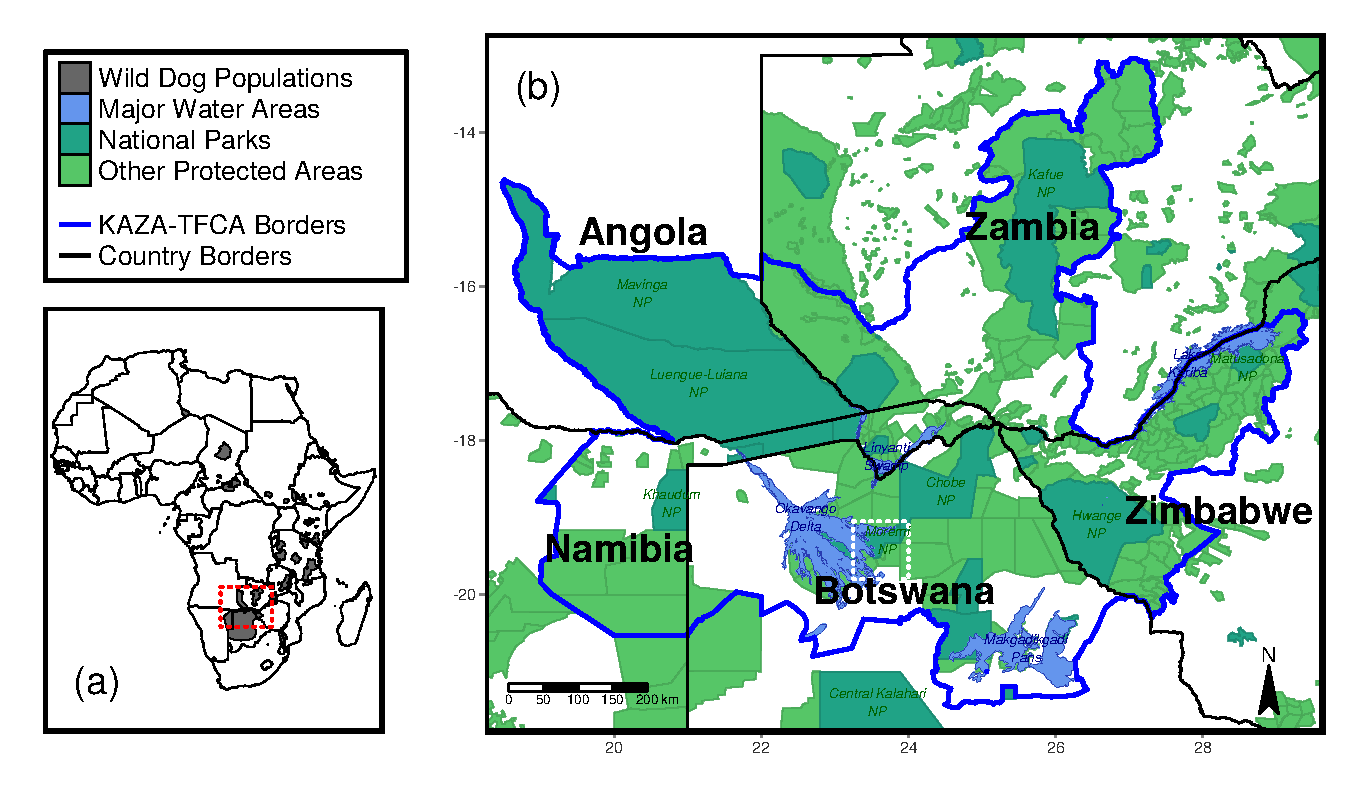
\includegraphics[width = \textwidth]{99_StudyArea.png}
  \caption{(a) Study area from which data on dispersing AWDs was collected.
  Dispersal trajectories are plotted in dark gray. The study area encompassed
  parts of the Okavango Delta, a highly dynamic, flood-pulse-driven ecosystem.
  The entire study area undergoes substantial seasonal changes, as can be seen
  from two satellite images taken during peak dry season (b1) and peak rainy
  season (b2). Notably, the flood of the Okavango Delta reaches its maximum
  extent during peak dry season.}
  \label{StudyArea}
 \end{center}
\end{figure}

\subsection{GPS Data}
Between the years 2015 and 2022, we collected GPS data of
\inputy{99_GeneralMetrics/CollarsTotal} dispersing AWD coalitions
(\inputy{99_GeneralMetrics/CollarsFemales} female coalitions,
\inputy{99_GeneralMetrics/CollarsMales} male coalitions) from a free-ranging
population in northern Botswana. Details on the GPS collar fitting procedure and
how we distinguished between dispersal and resident movements can be found in
\cite{Cozzi.2020} and \cite{Hofmann.2021}. During dispersal, we programmed GPS
satellite collars to record a GPS fix at a predetermined 4-hourly schedule. The
collars regularly transmitted the data to a base station, which allowed us to
track dispersing individuals, even if they moved outside the main study area. In
total, we successfully collected \inputy{99_GeneralMetrics/FixesTotal} fixes
during dispersal, with an average of \inputy{99_GeneralMetrics/FixesMeanSD}
fixes per coalition. Occasionally, the acquisition of a GPS location failed
(success rate = \inputy{99_GeneralMetrics/AcquisitionRate}\%), resulting in
irregular durations between some subsequent fixes.

\subsection{Spatial Habitat Layers}
We represented the physical landscape through which dispersers could move by a
series of spatial layers that we believed whould influence wild dog movements
during dispersal. The layers can be broadly categorized into descriptors of (1)
landscape characteristics, (2) climatic conditions, and (3) anthropogenic
factors (\Cref{tab:Covariates}). To appropriately render seasonal dynamicity in
each of these layers, we downloaded spatial data at the highest temporal
resolution available. That is, whenever possible, we represented covariates by a
series of raster layers that spanned the entire range of dates for which we
collected data of dispersing AWDs. We downloaded each product at the highest
spatial resolution available (\Cref{tab:Covariates}).

\begin{figure}
 \begin{center}
  \includegraphics[width = \textwidth]{99_SeasonalCovariates.png}
  \caption{Illustration of how some of the covariates considered in this study
  vary across seasons. Data for the graphs was obtained from the (a) Global
  Satellite Mapping of Precipitation dataset, (b) ERA5 dataset, (c) MODIS
  MOD13Q1 dataset, and (d) remote sensed MOD43A4 satellite images. Values were
  extracted across the study area and averaged by months. The smoothing curves
  were fitted using simple GAM models in the \texttt{mgcv} package
  \citep{Wood.2011}.}
  \label{Seasonality}
 \end{center}
\end{figure}

\inputy{99_Covariates.tex}

\subsubsection{Landscape Characteristics}
We used data from the MODIS Vegetation Continuous Fields dataset (MOD44B V061,
\citealp{DiMiceli.2022}) to represent vegetation across the study area. The
MOD44B dataset comprises three continuous layers, depicting the percentage cover
of \textsf{woodland}, \textsf{shrubs/grassland}, and \textsf{bareland},
respectively. Because the layers add up to 100\%, we only considered the two
layers \textsf{woodland} and \textsf{shrubs/grassland}, thus preventing issues
of perfect multicollinearity. This specific product is updated on day 65 of each
year and so we used the R-package \texttt{RGISTools} \citep{Perez-Goya.2020} to
download yearly updated layers for the years for which GPS data was at our
disposal. We also downloaded information on the normalized vegetation difference
index (NDVI) from the MODIS MOD13Q1 dataset \citep{Didan.2015}. This product is
updated every 16 days and we accessed the respective layers through Google Earth
Engine \citep{Gorelick.2017} using the r-package \texttt{rgee}
\citep{Aybar.2023}. We depicted open water sources using the Globeland30
dataset, from which we only retained the land-cover class water. To dynamically
update the distribution of floodwater across the extent of the Okavango Delta,
we combined the Globeland30 water-cover layer with weekly updated floodmaps
derived from remote sensed MODIS MOD43A4 satellite images. The algorithm upon
which the separation between floodwater and dryland is based is described in
detail in \cite{Wolski.2017} and \cite{Hofmann.2021} and is implemented in the
\texttt{floodmapr} package (available on GitHub;
\url{https://github.com/DavidDHofmann/floodmapr}). Because this algorithm has
been developed to remote sense large-scale bodies of floodwater, it is
unsuitable for the detection of smaller waterbodies, such as those represented
by pans. As such, we parametrized a classifier that was specifically focused on
detecting surface water from small-scale pans using Sentinel 2 satellite imagery
\citep{EuropeanSpaceAgency.2018}. This allowed us to obtain updated maps for the
distribution of pan-water at an interval of 5 to 10 days.

\subsubsection{Climate Descriptors}
We downloaded hourly updated information on above-ground temperature and
precipitation through Google Earth Engine \citep{Gorelick.2017} using the
\texttt{rgee} package \citep{Aybar.2023}. We obtained temperature data from the
ERA5-Land dataset \citep{Munoz-Sabater.2021}, whereas we utilized the Global
Satellite Mapping of Precipitation dataset to access precipitation data
\citep{Kubota.2020}. To match hourly values from the temperature and
precipitation data with the 4-hour fixes from the GPS data collection, we
computed average precipitation and temperature values across four hours.

\subsubsection{Anthropogenic Features}
We combined anthropogenic pressures arising from the presence of humans,
agriculture, and roads into a single proxy for human influence. We obtained
information on human density from Facebook's high resolution human density
dataset \citep{Tiecke.2017} which we downloaded from the humdata website
(\url{www.data.humdata.org/}). We also downloaded rasterized information on the
presence of agricultural fields from the Globeland30 \citep{Chen.2015} and
Cropland \citep{Xiong.2017} datasets. Vectorized data on main tar roads was
downloaded from OpenStreetMaps \citep{OpenStreetMapContributors.2017}. How the
individual layers were merged and combined into a single layer is described in
detail in \cite{Hofmann.2021}. Finally, we also derived vector data on the
distribution of national parks, wildlife management areas and other protected
areas from the Peace Parks Foundation (\url{www.maps.ppf.org.za/}).

\subsection{Step Selection Function}
We estimated seasonal habitat and movement preferences of dispersing individuals
using an integrated step-selection function (iSSF, \citealp{Fortin.2005,
Avgar.2016}). In iSSFs, \textit{observed} steps (i.e. the straight line between
two consequtive GPS locations \citep{Turchin.1998}) are compared to
\textit{random} steps in a conditional logistic regression framework
\citep{Fortin.2005, Thurfjell.2014, Muff.2020, Fieberg.2021}. We thus converted
subsequent GPS locations during dispersal into bursts of steps with equal
duration. For this, we first identified bursts of consecutive GPS fixes where
the duration between two GPS fixes did not exceed 4 hours (\(\pm\) 15 minutes).
Within each burst, we computed step lengths (sl) and relative turning angles
(ta) associated with each observed step. \inputy{99_GeneralMetrics/SSFTotal}
dispersing coalitions (\inputy{99_GeneralMetrics/SSFFemales} female coalitions,
\inputy{99_GeneralMetrics/SSFMales} male coalitions) remained in the final
dataset. This yielded a total of \inputy{99_GeneralMetrics/StepsTotal} steps
(\inputy{99_GeneralMetrics/StepsMeanSD} per coalition). We partitioned the
resulting steps into wet and dry season.
\inputy{99_GeneralMetrics/PercentageStepsDry}\% of the GPS data fell into the
dry season, \inputy{99_GeneralMetrics/PercentageStepsWet}\% into the wet-season.

We paired each observed step with a set of 25 random steps, generated by
sampling turning angles from  a uniform distribution U(\(-\pi, +\pi\)) and step
lengths from a gamma distribution fitted to observed steps (scale \(\theta\) =
valuefromtex and shape \(k\) = valuefromtex) using the \texttt{fitdistrplus}
package \citep{Delignette-Muller.2015}. Together, an observed step and its 25
associated random steps formed a stratum that received a unique identifier.
Along each step, we extracted covariate values from the underlying spatial
habitat layers (\Cref{tab:Covariates}). For continuous covariates, we computed
average values along each step, for categorical covariates the percentage cover
of each category along the step. To facilitate model convergence, we
standardized extracted values using a z-score transformation.

We then assumed that each animal assigned a score \(w(x)\) of the following
exponential form to each realized and random step \citep{Fortin.2005}:

\begin{equation}
\label{EQ1}
  w(x) = exp(\beta_1 x_1 + \beta_2 x_2 + ... + \beta_n x_n)
\end{equation}

\noindent Here, (\(x_1, x_2, ..., x_n\)) represent the covariate values along
the respective step and (\(\beta_1, \beta_2, ..., \beta_n\)) are the animal's
relative selection strengths \citep{Avgar.2017} towards these covariates. To
estimate relative selection strengths (i.e. the \(\beta\)'s), we used the mixed
effects conditional logistic regression model as proposed by \cite{Muff.2020}.
We implemented their method using the R-package \textit{glmmTMB}
\citep{Brooks.2017} and used dispersing coalition ID to model random slopes. The
approach also requires the inclusion of a random intercept with an arbitrarily
fixed variance of 10\textsuperscript{6}.

To establish whether the number of random steps sufficed to reliably estimate
model parameters, we ran a series univariate models where we only included
single predictors and estimated model coefficients considering 1, 5, 10, 50, and
100 random steps, respectively (sensu \citealp{Fieberg.2020}). We replicated
each model run 100 times and randomly resampled the necessary number of random
steps. This allowed us to investigate the minimum number of random steps that
were required before estimates for habitat and movement preferences converged
towards a stationary estimate.

\section{Results}

\begin{figure}
 \begin{center}
  \includegraphics[width = \textwidth]{99_MovementModel.png}
  \caption{This is a caption}
  \label{Movement Model}
 \end{center}
\end{figure}

\inputy{99_MovementModel.tex}

\section{Discussion}
Dynamic connectivity increases our understanding of temporal changes in
connectivity \citep{Martensen.2017}.

\cite{Martensen.2017} showed that dynamic connectivity was higher than static
connectivity because of stepping stones that emerged and disappeared again.

\cite{Osipova.2019} in contrast find that connectivity is both over and
underestimated, depending on the season.

\cite{Benz.2016} showed that habitat selection of moose changes depending on the
season and used a combination of RSFs and SSFs to study habitat selection across
seasons.

Badly designed corridors can result in population sinks and wasted financial
resources \citep{Simberloff.1992}.

Could talk a bit about the following papers: \citep{Chetkiewicz.2009, Benz.2016,
Mui.2017, Osipova.2019, Kaszta.2021}

\section{Authors' Contributions}
D.D.H. and G.C. conceived the study and designed methodology; D.D.H., G.C.,
D.M.B, and J.W.M. collected the data; D.D.H. analysed the data; G.C. assisted
with modeling; D.D.H. and G.C. wrote the first draft of the manuscript and all
authors contributed to the drafts at several stages and gave final approval for
publication.

\section{Data Availability}
GPS movement data of dispersing wild dogs is available on dryad
\citep{Hofmann.2021a}. Access to R-scripts that exemplify the application of the
proposed approach using simulated data are provided through Github
(\url{https://github.com/DavidDHofmann/DispersalSimulation}). In addition, all
codes required to reproduce the African wild dog case study will be made
available through an online repository at the time of publication.

\section{Acknowledgements}
We thank the Ministry of Environment and Tourism of Botswana for granting
permission to conduct this research. We thank C. Botes, I. Clavadetscher, and G.
Camenisch for assisting with wild dog immobilizations. We also thank B. Abrahms
for sharing her data of three dispersing wild dogs. Furthermore, we would like
to thank Johannes Signer for assisting with the simulation algorithm. This study
was funded by Albert-Heim Foundation, Basler Stiftung für Biologische Forschung,
Claraz Foundation, Idea Wild, Jacot Foundation, National Geographic Society,
Parrotia Stiftung, Stiftung Temperatio, Wilderness Wildlife Trust Foundation,
Forschungkredit der Universität Zürich, and a Swiss National Science Foundation
Grant (31003A\_182286) to A. Ozgul.

\newpage
\begingroup
\singlespacing

% \printbibliography
\bibliography{Literature}
\endgroup

\end{document}
